\section{Results Analysis - Linear Drag Model}
Prepare yourself, because our hard work has paid off.

\subsection{Test Case: High Drag}
We fit our linear drag model to the same test case as Fig.~\ref{fig:Analysis1_Test4_Fig5_NoDrag}, and the results are shown in Fig.~\ref{fig:Analysis2_Test4_Fig5_LinearDrag}. The position and velocity plots both track very nicely.\footnote{We provide no quantitative analysis of the fit here due to a lack of internalized, intuitive understanding of statistics. I'm not going to show numbers for the sake of showing numbers if they don't mean anything to me. In my professional experience, people have relied on me to judge if the vibes are good or bad without ever asking me for the numbers to prove it.}

The more interesting results are in the frame-by-frame behavior.

\begin{figure}[t]
\centering
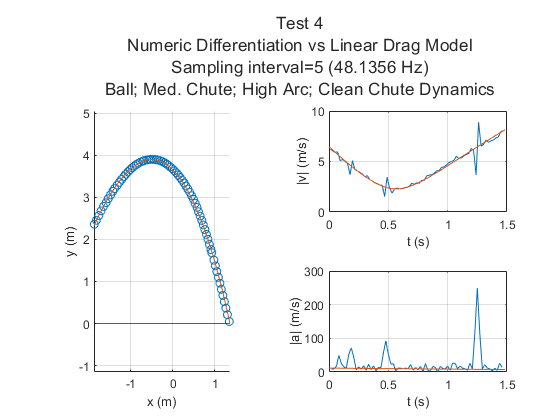
\includegraphics[width=0.9\linewidth]{images/Analysis2_Test4_Fig5_LinearDrag.png}
\caption{\label{fig:Analysis2_Test4_Fig5_LinearDrag} Fitting the linear drag model to sampled position data for a ball with a parachute. Lookin' good. Check out how nice it tracks the velocity plot while rejecting the spikes.}
\end{figure}

\subsection{Test Case: High Drag - Frame by Frame}

\begin{figure*}[t!]
    \centering
    \begin{subfigure}[t]{0.5\textwidth}
        \centering
        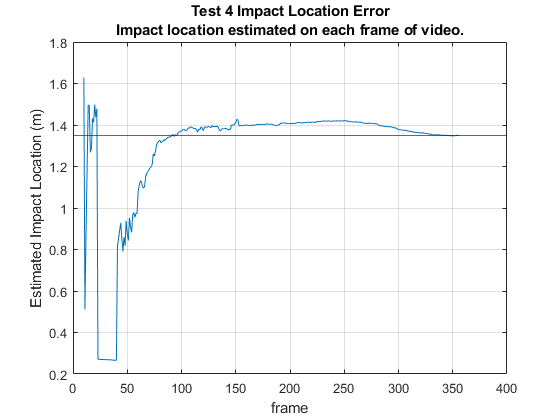
\includegraphics[width=\textwidth]{images/Analysis2_Test4_ImpLocPlot_LinearDrag.png}
        \caption{}
    \end{subfigure}%
    ~ 
    \begin{subfigure}[t]{0.5\textwidth}
        \centering
        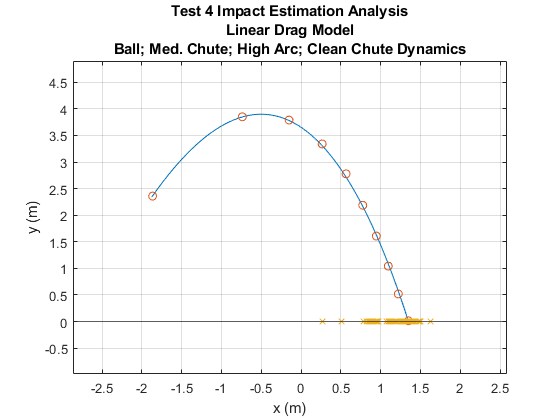
\includegraphics[width=\textwidth]{images/Analysis2_Test4_ImpLocHist_LinearDrag.png}
        \caption{}
    \end{subfigure}
    \caption{\label{fig:Test4_LinearDrag_FrameByFrame} Frame-by-frame impact location estimation for a ball with a parachute using the linear drag model. (a) Impact location over time. (b) Impact locations marked.}
\end{figure*}

Now Fig.~\ref{fig:Test4_LinearDrag_FrameByFrame} is some data you can sink your teeth into. 